\documentclass[corpo=12pt,twoside,tipotesi=magistrale,stile=classica]{toptesi}
\usepackage[english,italian]{babel}
\usepackage[utf8]{inputenc}
\usepackage[autostyle]{csquotes}
\usepackage[backend=biber]{biblatex}
\usepackage[]{hyperref}
\usepackage{lipsum}
\usepackage{comment}


\addbibresource{Bibliografia/bibliografia.bib}

\hypersetup{
	colorlinks=true,
	linkcolor=black,
	filecolor=magenta,      
	urlcolor=cyan,
}

\includecomment{it}
\excludecomment{en}

%\includecomment{en}
%\excludecomment{it}


\begin{document}
\begin{en}
	\english
	\begin{frontespizio*}
		\ateneo{Politecnico di Torino}
		\logosede{polito}
		\CorsoDiLaureaIn{Master of Science’s Degree in}
		\corsodilaurea{Aerospace Engineering}	
		\TesiDiLaurea{Master's Thesis}	
		\titolo{Processor in the loop simulations and Code generation for Unmanned Aerial systems}
		\AdvisorName{Supervisor:}
		\relatore{Prof.ssa Elisa Capello}
		\CoAdvisorName{Co-supervisor}
		\secondorelatore{Dott. Davide Carminati}
		\sedutadilaurea{December 2020}
		\TitoloListaCandidati{Author:}
		\candidato{Luigi Sante}
	\end{frontespizio*}
\end{en}

\begin{it}
	\begin{frontespizio*}
		\ateneo{Politecnico di Torino}
		\logosede{polito}
		\CorsoDiLaureaIn{Laurea Magistrale in}
		\corsodilaurea{Ingegneria Aerospaziale}	
		\TesiDiLaurea{Tesi Magistrale}	
		\titolo{Processor in the loop simulations and Code generation for Unmanned Aerial systems}
		\AdvisorName{Relatore:}
		\relatore{Prof.ssa Elisa Capello}
		\CoAdvisorName{Co-Relatore}
		\secondorelatore{Dott. Davide Carminati}
		\sedutadilaurea{Dicembre 2020}
		\TitoloListaCandidati{Autore:}
		\candidato{Luigi Sante}
	\end{frontespizio*}
\end{it}

	
	\sommario
	TODO : Parlare di cosa tratta la tesi
	\ringraziamenti
	TODO : Scrivere i ringraziamenti
	
	
	\tableofcontents
	\listoftables
	\listoffigures
	
	\mainmatter
	
	\begin{it}
	\chapter{PX4 Autopilot}
	Il firmware utilizzato nelle simulazioni di software in the loop e processor in the loop è il PX4 Autopilot.
		
	Questo software mette a disposizione diverse funzionalità per avere un sistema di gestione e controllo robusto è affidabile implementato in diversi tipi di sistemi. L'implementazione non è quindi specifica solo a mezzi aerei di qualsiasi configurazione, ma anche a velivoli di terra e marini. Il software è open-source è vanta del contributo di parecchi sviluppatori, dagli esperti del settore a contributi di livello accademico. Lo sviluppo open-source permette quindi di aggiungere o modificare le funzionalità messe a disposizione. Il sistema operativo sulla quale viene eseguito materialmente il codice può essere Nuttx o Linux/MacOS la cui distinzione è solo nella gestione di task e thread.
	
	Il sistema operativo Nuttx è un sistema RTOS (Real-Time Operating System) è svilupato appositamente per implementazioni embedeed. Essendo sviluppato per un contesto specifico ha tutte le caratteristiche necessarie per essere eseguito in sistemi che devono avere prestazioni migliori con poche risorse disponibili. Vengono utilizzati gli standard POSIX e ANSI. Inoltre, sono implementate funzionalità di programmazione concorrenziale per l'esecuzione di processi in parallelo. Le funzionalità del firmware vengono eseguite in questo sistema come task separati e ogni task può eseguire diversi thread.
	Nell'implementazione su sistemi Linux/MacOS invece i moduli sono eseguiti come thread del processo principale, non c'è quindi una distinzione tra threads e tasks.
\end{it}

\begin{en}
	\chapter{PX4 Autopilot firmware}
	The firmware used to run the software in the loop and the processor in the loop simulations is the PX4 Autopilot.
	
	This software provides various functionalities to have a robust and reliable management and control system implemented in different types of systems. The implementation is therefore not specific only to aircraft of any configuration, but also to land and marine aircraft. The software is open-source and boasts contributions from several developers, from industry experts to academic-level contributions. Open-source development therefore allows you to add or modify the functionalities made available. The operating system on which the code is physically executed can be Nuttx or Linux/MacOS whose distinction is only in the management of tasks and threads.
	
	The Nuttx operating system is a Real-Time Operating System (RTOS) that is specially developed for embedeed implementations. Being developed for a specific context it has all the features necessary to run on systems that need to have better performance with few resources available. POSIX and ANSI standards are used. In addition, concurrent scheduling capabilities are implemented for running processes in parallel. Firmware features run in this system as separate tasks, and each task can execute several threads.
	In the implementation on Linux/MacOS systems, on the other hand, modules are executed as threads of the main process, so there is no distinction between threads and tasks.
\end{en}

\begin{it}
	\section{Architettura del software}
	Il firmware è principalmente suddiviso in due categorie di moduli:
	\begin{itemize}
		\item \textbf{Flight stack} : composta dalla parte che stima lo stato del sistema e il relativo controllo
		\item \textbf{Middleware} : composta dalle interfacce che collegano i vari moduli interni di PX4 tra di loro e verso l'esterno, con la possibilità di integrare gli hardware utilizzati.
	\end{itemize}
	
	Il sistema quindi separa le varie funzionalità in moduli separati, eseguiti in modo indipendente che scambiano i dati e comandi tra di loro e con l'esterno attraverso messaggi asincroni.
	Nella figura \ref{fig:px4.architettura} è riportato lo schema di alto livello del software di PX4 e la sua modularità.
	
	\begin{figure}[ht]
		\centering
		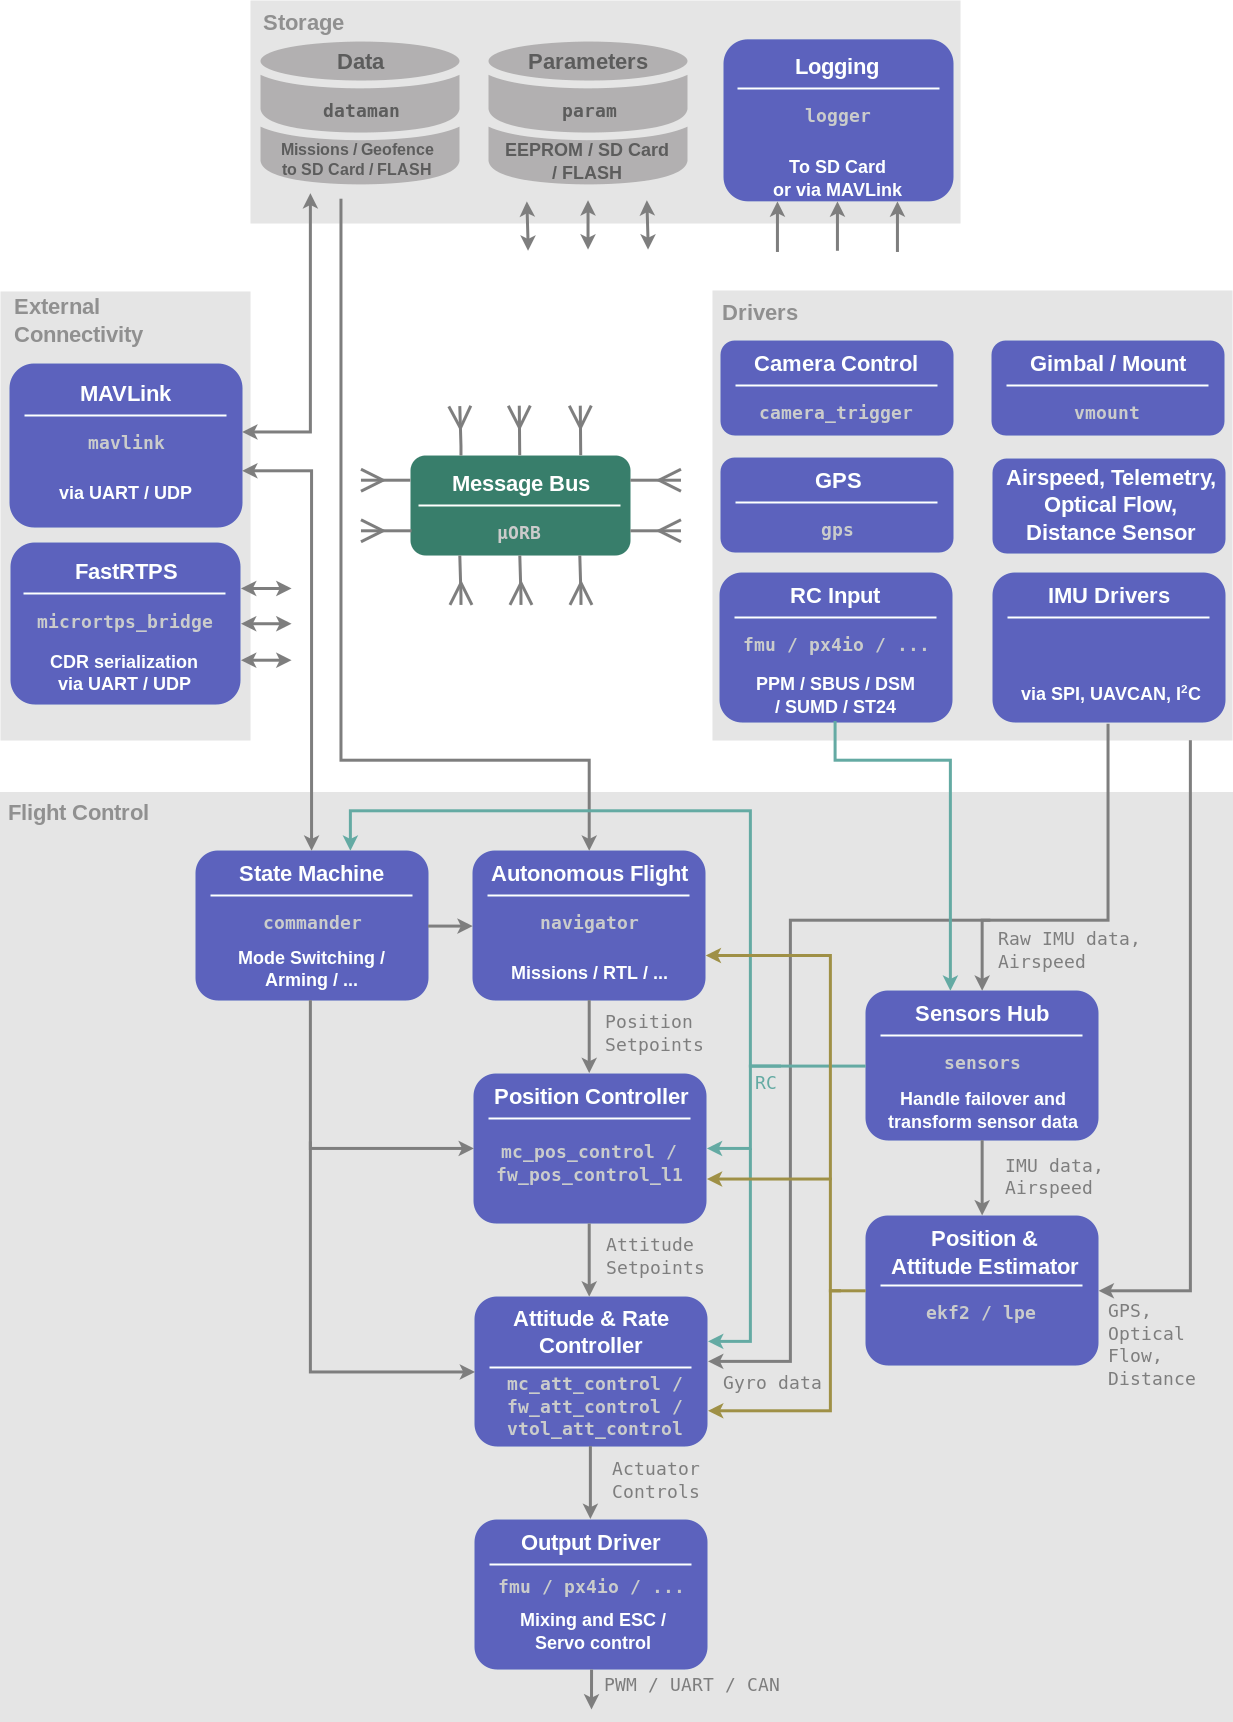
\includegraphics[width=1\textwidth]{Contestualizzazione/Figure/PX4_Architecture}
		\caption{Architettura del codice di PX4 Autopilot}
		\label{fig:px4.architettura}
	\end{figure}
	\subsection{Flight stack}
	Il flight stack, mostrato in figura \ref{fig:px4.flightstack} è l'insieme di moduli che si occupano della stima dello stato del sistema e di tutti le funzionalità per il controllo,la guida e la navigazione. Esiste anche un modulo per interfacciarsi con il volo manuale attraverso radiocomando.
		\begin{figure}[ht]
		\centering
		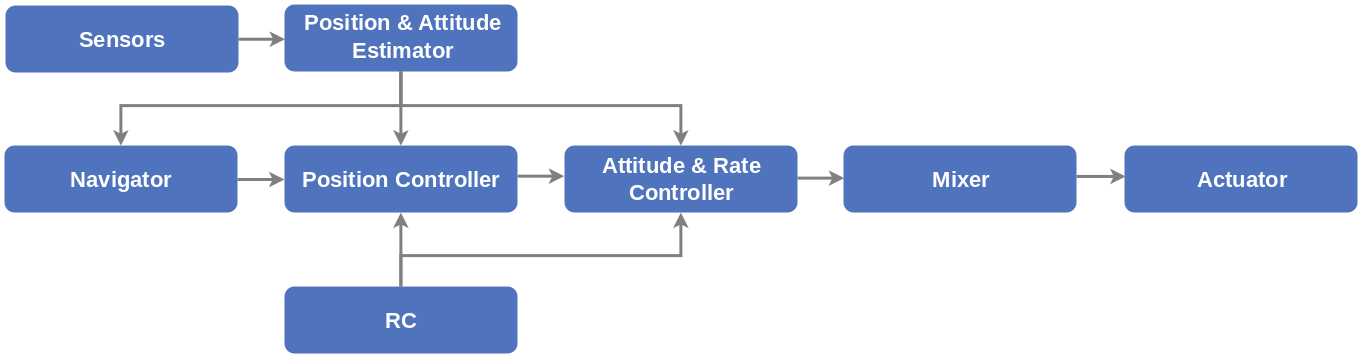
\includegraphics[width=1\textwidth]{Contestualizzazione/Figure/PX4_High-Level_Flight-Stack}
		\caption{Architettura del flight stack di PX4}
		\label{fig:px4.flightstack}
	\end{figure}
	\paragraph{Sensors}
		Da dove prende i dati?
		Che cosa fa?
		A cosa serve?
	  	Per chi lo fa?
	\paragraph{Position \& Attitude Estimator}
	\paragraph{Navigator}
	\paragraph{Position Controller}
	\paragraph{Attitude \& Rate Controller}
	\paragraph{Mixer}
	\paragraph{Actuator}
	\paragraph{RC}
	
	
	
\end{it}

\begin{en}
	\section{Software Architecture}
	Come è strutturato il software?
	
	Suddivisione per funzionalita?
	Quali sono le funzionalità interne dei vari moduli?
	Come sono collegati i vari moduli?
	Come avviene l'interfacciamento con i sensori?
	Come avviene l'interfacciamento con il simulatore?
	
	Perchè viene utilizzato questo firmware?
	Quali sono gli strumenti messi a disposizione per lo sviluppo?
	Parlare della compilazione base del firmware attraverso il codice
	Parlare della compilazione attraverso il tool di MATLAB 
	Quali moduli vengono sostituiti nel firmware?
\end{en}
	
	
%	\appendix
	
	
	\backmatter
	\nocite{*}
\printbibliography[heading=bibintoc]
	
\end{document}